\documentclass[a4paper]{article}
\usepackage[utf8]{inputenc}
\usepackage[spanish, es-tabla, es-noshorthands]{babel}
\usepackage[table,xcdraw]{xcolor}
\usepackage[a4paper, footnotesep = 1cm, width=18cm, left=2cm, top=2.5cm, height=25cm, textwidth=18cm, textheight=25cm]{geometry}
%\geometry{showframe}

\usepackage{amsmath}
\usepackage{amsfonts}
\usepackage{amssymb}
\usepackage{float}
\usepackage{graphicx}
\usepackage{caption}
\usepackage{subcaption}
\usepackage{multicol}
\usepackage{multirow}
\setlength{\doublerulesep}{\arrayrulewidth}

\graphicspath{{../Ejercicio-1/}{../Ejercicio-2/}{../Ejercicio-3y4/}{../Ejercicio-5-6y7/}{../Ejercicio-8/}}

\usepackage{hyperref}
\hypersetup{
    colorlinks=true,
    linkcolor=blue,
    filecolor=magenta,      
    urlcolor=blue,
    citecolor=blue,    
}
\newcommand\underrel[2]{\mathrel{\mathop{#2}\limits_{#1}}}
\newcommand{\quotes}[1]{``#1''}
\usepackage{array}
\newcolumntype{C}[1]{>{\centering\let\newline\\\arraybackslash\hspace{0pt}}m{#1}}
\usepackage[american,oldvoltagedirection,siunitx]{circuitikz}
\usepackage{fancyhdr}
\usepackage{units}
\usepackage{booktabs}

\usepackage{tikz}
\usetikzlibrary{babel}

\pagestyle{fancy}
\fancyhf{}
\lhead{22.42 Laboratorio de Electrónica}
\rhead{Bertachini, Lambertucci, Londero Bonaparte, Mechoulam, Scapolla}
\rfoot{\center \thepage}

\begin{document}
\section{Puente de Wien - Medición de frecuencias}

\subsection{Introducción}
En esta sección, se procederá a diseñar un puente de Wien, analizando las sensibilidades para todo el rango de medición. \par
Dicho puente permitirá conocer la frecuencia de una fuente desconocida, esto se debe a un procedimiento por el cual se comparan distintas magnitudes presentes en las ramas del puente, se puede considerar como un proceso de medición indirecta. Existen limitaciones de tipo constructivas para el rango de frecuencias que se pueden medir, el asignado por la cátedra es de $10KHz$ a $200KHz$.\par
Un puente se considera en equilibrio cuando ocurren dos circunstancias en simultáneo, en primer lugar, cuando el cociente entre la tensión en la salida del puente $V_D$ y la tensión del generador $V_G$ es nulo, por otro lado, el cociente entre una impedancia y su opuesta debe ser equivalente al otro par dentro del circuito. La primer hipótesis nunca se podrá confirmar ya que es una afirmación de carácter netamente teórico, en la práctica nunca se obtendrá una tensión nula debido tanto a la incerteza en los métodos de medición utilizados, mostrado en el ejercicio 1, así como también a las sensibilidades propias de los componentes. \par
El puente de Wien cuenta con cuatro ramas, el primer par de ramas adyacentes cuentan con componentes puramente resistivos, el otro par está formado por circuitos RC, uno en paralelo y otro en serie, como se puede apreciar en el circuito [\ref{fig:Puente_de_wien}]. \par


%Puente_de_wien
\begin{figure}[H]
\centering
\includegraphics[scale=0.7]{Circuitos/Puente_de_Wien.pdf}
\caption{Puente de Wien planteado}
\label{fig:Puente_de_wien}
\end{figure}
%~Puente_de_wien


Las relaciones obtenidas para el mismo en condición de equilibrio son las siguientes: \par
\begin{equation}
\frac{R_1}{R_3}+\frac{C_3}{C_1}=\frac{R_2}{R_4}
\end{equation}
\begin{equation}
w=\frac{1}{\sqrt{C_1C_3R_1R_3}}
\end{equation} \par
Generalmente, y esa es la manera en la que se procederá en este trabajo, el diseño del puente se realiza considerando las frecuencias desconocidas de las fuentes a medir. Se fijarán valores equivalentes para los capacitores, lo mismo sucederá con sus resistencias asociadas. 
\begin{equation}
R_1=R_3=R \quad	\wedge \quad C_1=C_3=C
\end{equation}
Dando como resultado, la siguiente relación para las ramas puramente resistivas:
\begin{equation}
R_2=2R_4
\end{equation}
Reduciendose el cálculo de la frecuencia a:
\begin{equation}
f=\frac{1}{2\pi RC}
\label{frec}
\end{equation}
Las resistencias relacionadas con los capacitores son las que serán variadas para definir el comportamiente del puente, las mismas tendrán una sensibilidad asociada. Con dicha finalidad, se utilizarán resistencias variables de precisión (preset multivueltas de 25 vueltas). 

Partiendo de la fórmula para la sensibilidad dada por $\Delta V_D=V_GF\delta_{Z_i}=V_GF\frac{\Delta Z_i}{Z_i}$ siendo $i$ la i-ésima rama, se obtendrán las siguientes sensibilidades para las resistencias variables $R_3$ y $R_1$.
\begin{equation}
\Delta V_{D_{R_1}}=V_g\left|\frac{\$C_1R_1}{\$C_1R_1+1}\right|\frac{\Delta R_1}{R_1}
\label{VDR1}
\end{equation}
\begin{equation}
\Delta V_{D_{R_3}}=V_g\left|\$C_3R_3+1\right|\frac{\Delta R_3}{R_3}
\label{VDR3}
\end{equation}
Siendo $F$ el factor cabeza de puente dado por:
\begin{equation}
F=\frac{A}{1+2A\cos(\theta_A)+A^2} \quad \wedge \quad A=\frac{Z_4}{Z_2}
\label{cabeza_de_puente}
\end{equation} 

\subsection{Desarrollo}
Primeramente, como primera decisión de diseño se considera implementar dos presets por cada resistencia variable requerida. La implementación de dos componentes se debe a que uno serviría para ajuste grueso y el otro para un ajuste fino, logrando de esta manera obtener un ajuste más preciso que permita reducir la sensibilidad. Para los valores de frecuencia propuestos por la cátedra y usando un capacitor multicapa de $1nf$, era necesario lograr valores de resistividad entre los $800 \Omega$ y $16K\Omega$. En la práctica, no había disponibles en el pañol magnitudes de presets como para cubrir dicho rango, sin utilizar menos de 4 componentes, por lo que se decidió utilizar dos presets de $10K\Omega$.
\par 
Luego de investigar y simular para distintos valores, se decide tomar los siguientes valores para las ramas puramente resistivas del puente, $R_4=1K\Omega$ y $R_2=2K\Omega$. Volviendo a la ecuación [\ref{cabeza_de_puente}], obtendremos un valor cabeza de puente $A=\frac{1}{2}$, que dará un $F=0.22$.

Se obtienen las siguientes sensibilidades utilzando las fórmulas presentes en [\ref{VDR1}][\ref{VDR1}]:
%Sensibilidades
\begin{figure}[H]
\centering
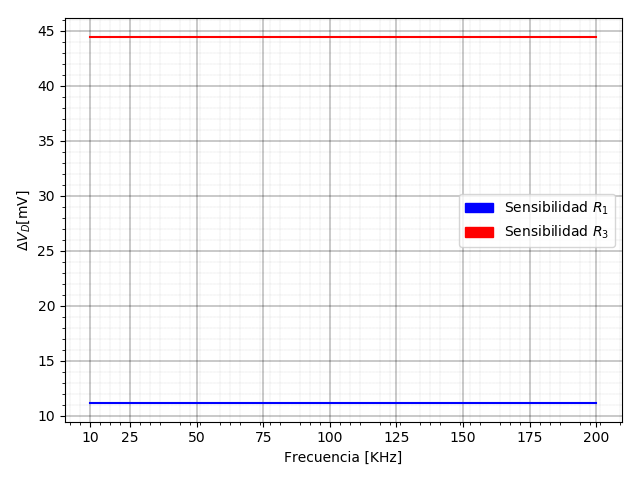
\includegraphics[scale=0.7]{Graficos/Sensibilidad}
\caption{Sensibilidades $R_1$ y $R_3$}
\label{fig:Sensibilidades}
\end{figure}
%~Sensibilidades

A continuación, se presenta el estudio del error al medir la frecuencia.

\begin{table}[H]
\centering
\begin{tabular}{ccccc}
\hline
$\mathbf{f_g \ [kHz]}$ & $\mathbf{P_{R1} + P_{R2} \ [k\Omega]}$ & $\mathbf{P_{R3} + P_{R4} \ [k\Omega]}$ & $\mathbf{f_c \ [kHz]}$ & \textbf{Error [\%]} \\
\hline
10                     & 15.16                                  & 15.92                                  & 10.24                  & 2.45                \\
21.14                  & 7.53                                   & 7.95                                   & 20.57                  & 2.70                \\
44.7                   & 3.56                                   & 3.75                                   & 43.56                  & 2.55                \\
65.01                  & 2.58                                   & 2.45                                   & 63.30                  & 2.63                \\
94.55                  & 1.68                                   & 1.74                                   & 93.09                  & 1.55                \\
137.27                 & 1.159                                  & 1.187                                  & 135.69                 & 1.15                \\
165.69                 & 0.961                                  & 0.985                                  & 163.58                 & 1.27                \\
200                    & 0.8                                    & 0.82                                   & 196.98                 & 1.51   				\\
\hline            
\end{tabular}
\caption{Error entre frecuencia del generador y calculada}
\label{tab:Tabla_error}
\end{table}

%Tension 10KHz
\begin{figure}[H]
\centering
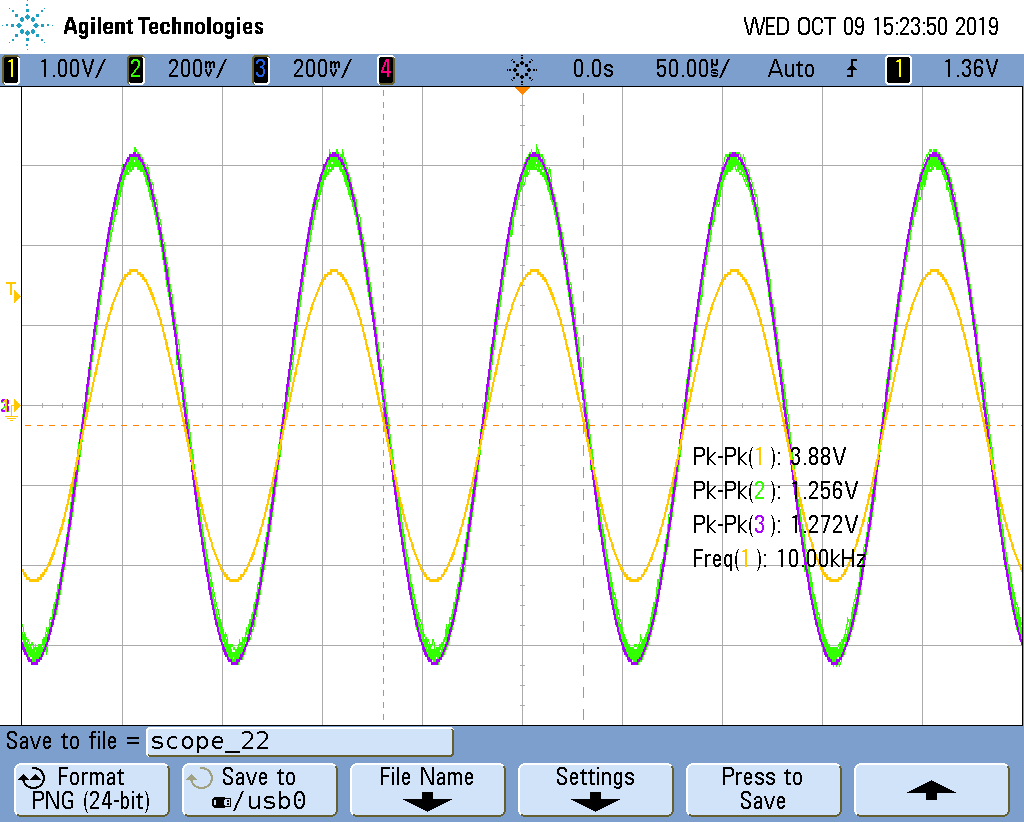
\includegraphics[width=0.8\textwidth,trim={0.25cm 5cm  1 5cm},clip]{Mediciones/Tensiones_10_KHz}
\caption{Tensión en $V_D$ a 10 KHz}
\label{fig:Tensiones_10_KHz}
\end{figure}
%~Tension 10KHz

%Tension 200KHz
\begin{figure}[H]
\centering
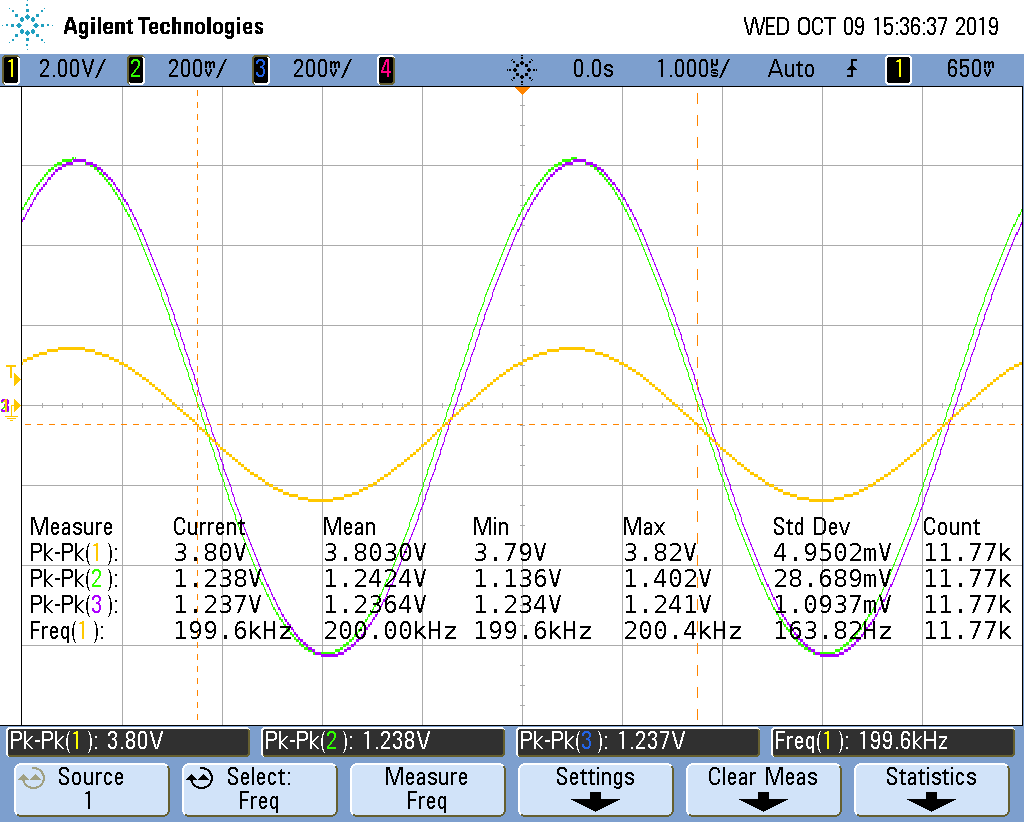
\includegraphics[width=0.8\textwidth,trim={0.25cm 5cm  1 5cm},clip]{Mediciones/Tensiones_200_KHz}
\caption{Tensión en $V_D$ a 200 KHz}
\label{fig:Tensiones_200_KHz}
\end{figure}
%~Tension 200KHz


\subsection{Conclusiones}

En la práctica, las resistencias que se suponían de igual magnitud como una condición inicial ($R_3$ y $R_1$) dejarán de serlo como se puede apreciar en [\ref{tab:Tabla_error}] planteada en el desarrollo, esto se debe a la variación que hay que introducir en las magnitudes de los presets para poder llegar lo más cercano posible a la condición de equilibrio($V_D=0$) considerando las sensibilidades previamente calculadas.
Por otro lado, se observa que el error obtenido para el cálculo de la frecuencia es  considerablemente bajo[\ref{tab:Tabla_error}], con un promedio de 1.97\%. Consecuentemente, se buscó si existían otros valores de resistencias, bajo la misma frecuencia, con los que se pudiese llegar a la condición de equilibrio, descubriéndose que existen dichos valores pero el error es considerablemente más alto, entre el \%25 y \%50 generalmente. Dicha mayor diferencia en el error, se debe a que la diferencia entre las resistencias se volvía considerablemente mayor, llegando en algunos casos a un orden de magnitud. 
\end{document}